\iffalse
\documentclass[12pt]{article}
\usepackage{graphicx}
\usepackage{commath}
\usepackage{gensymb}

\begin{document}
\begin{center}
\textbf\large{CHAPTER-10 \\ VECTOR ALGEBRA}
\end{center}

\section{EXERCISE - 10.3}
\begin{enumerate}
		\fi
\begin{enumerate}[label=\thesection.\arabic*,ref=\thesection.\theenumi]
\item Find the angle between two vectors $\overrightarrow{a}$ and $\overrightarrow {b} $ with magnitudes $\sqrt{3}$ and 2 respectively having $\overrightarrow {a}.\overrightarrow {b}=\sqrt{6}$.
\item Find the angle between the the vectors $\hat{i}-2\hat{j}+3\hat{k}$ and $3\hat{i}-2\hat{j}+\hat{k}$.
\item Find the projection of the vector $\hat{i}-\hat{j}$ on the vector $\hat{i}+\hat{j}$.
	\\
		\iffalse
\documentclass[12pt]{chapters/10/7/4/3/figsarticle}
\usepackage{graphicx}
\usepackage[none]{chapters/10/7/4/3/figshyphenat}
\usepackage{graphicx}
\usepackage{listings}
\usepackage[english]{chapters/10/7/4/3/figsbabel}
\usepackage{graphicx}
\usepackage{caption} 
\usepackage{booktabs}
\usepackage{array}
\usepackage{amssymb} % for \because
\usepackage{amsmath}   % for having text in math mode
\usepackage{extarrows} % for Row operations arrows
\usepackage{listings}
\lstset{
  frame=single,
  breaklines=true
}
\usepackage{hyperref}
  
%Following 2 lines were added to remove the blank page at the beginning
\usepackage{atbegshi}% http://ctan.org/pkg/atbegshi
\AtBeginDocument{\AtBeginShipoutNext{\AtBeginShipoutDiscard}}


%New macro definitions
\newcommand{\mydet}[1]{chapters/10/7/4/3/figs\ensuremath{\begin{vmatrix}#1\end{vmatrix}}}
\providecommand{\brak}[1]{chapters/10/7/4/3/figs\ensuremath{\left(#1\right)}}
\newcommand{\solution}{\noindent \textbf{Solution: }}
\newcommand{\myvec}[1]{chapters/10/7/4/3/figs\ensuremath{\begin{pmatrix}#1\end{pmatrix}}}
\providecommand{\norm}[1]{chapters/10/7/4/3/figs\left\lVert#1\right\rVert}
\providecommand{\abs}[1]{chapters/10/7/4/3/figs\left\vert#1\right\vert}
\let\vec\mathbf


\begin{document}

\begin{center}
\title{\textbf{VECTORS}}
\date{\vspace{-5ex}} %Not to print date automatically
\maketitle
\end{center}

\setcounter{page}{1}

\section{10$^{th}$ Maths - Chapter 10}

This is Problem-3 from Exercise 10.3

\begin{enumerate}
\item Find the projection of the vector $\hat{i}-\hat{j}$ on the vector $\hat{i}+\hat{j}$  
\end{enumerate}
\section{SOLUTION}
\fi
\solution
The given points are
\begin{align}
 \vec{A}=\myvec{1\\ -1},
 \vec{B}=\myvec{1\\ 1}
\end{align}
Since
\begin{align}
	\vec{A}^\top \vec{B} &= \myvec{1 &-1} \myvec{1\\ 1}=\myvec{1 \times 1}+\myvec{-1 \times  1}=0
	\\
	\norm {\vec {B}}^2 &= (\vec{B}^\top  \vec{B})=\myvec{1 & 1} \myvec{1\\ 1}= (1 \times  1)+(1 \times  1)=2,
\end{align}
and the project vector is given by 
\begin{align}
	\vec{C} &= 
	\frac{\vec{A}^\top  \vec{B}}{\norm {\vec{B}}}^2 \vec{B}
	&=\frac{0}{2} \myvec{1\\ 1}
	=\myvec{0\\ 0}
\end{align}
This is verfied in Fig.
		\ref{fig:12/10/3/3Figure}.
\begin{figure}[h]
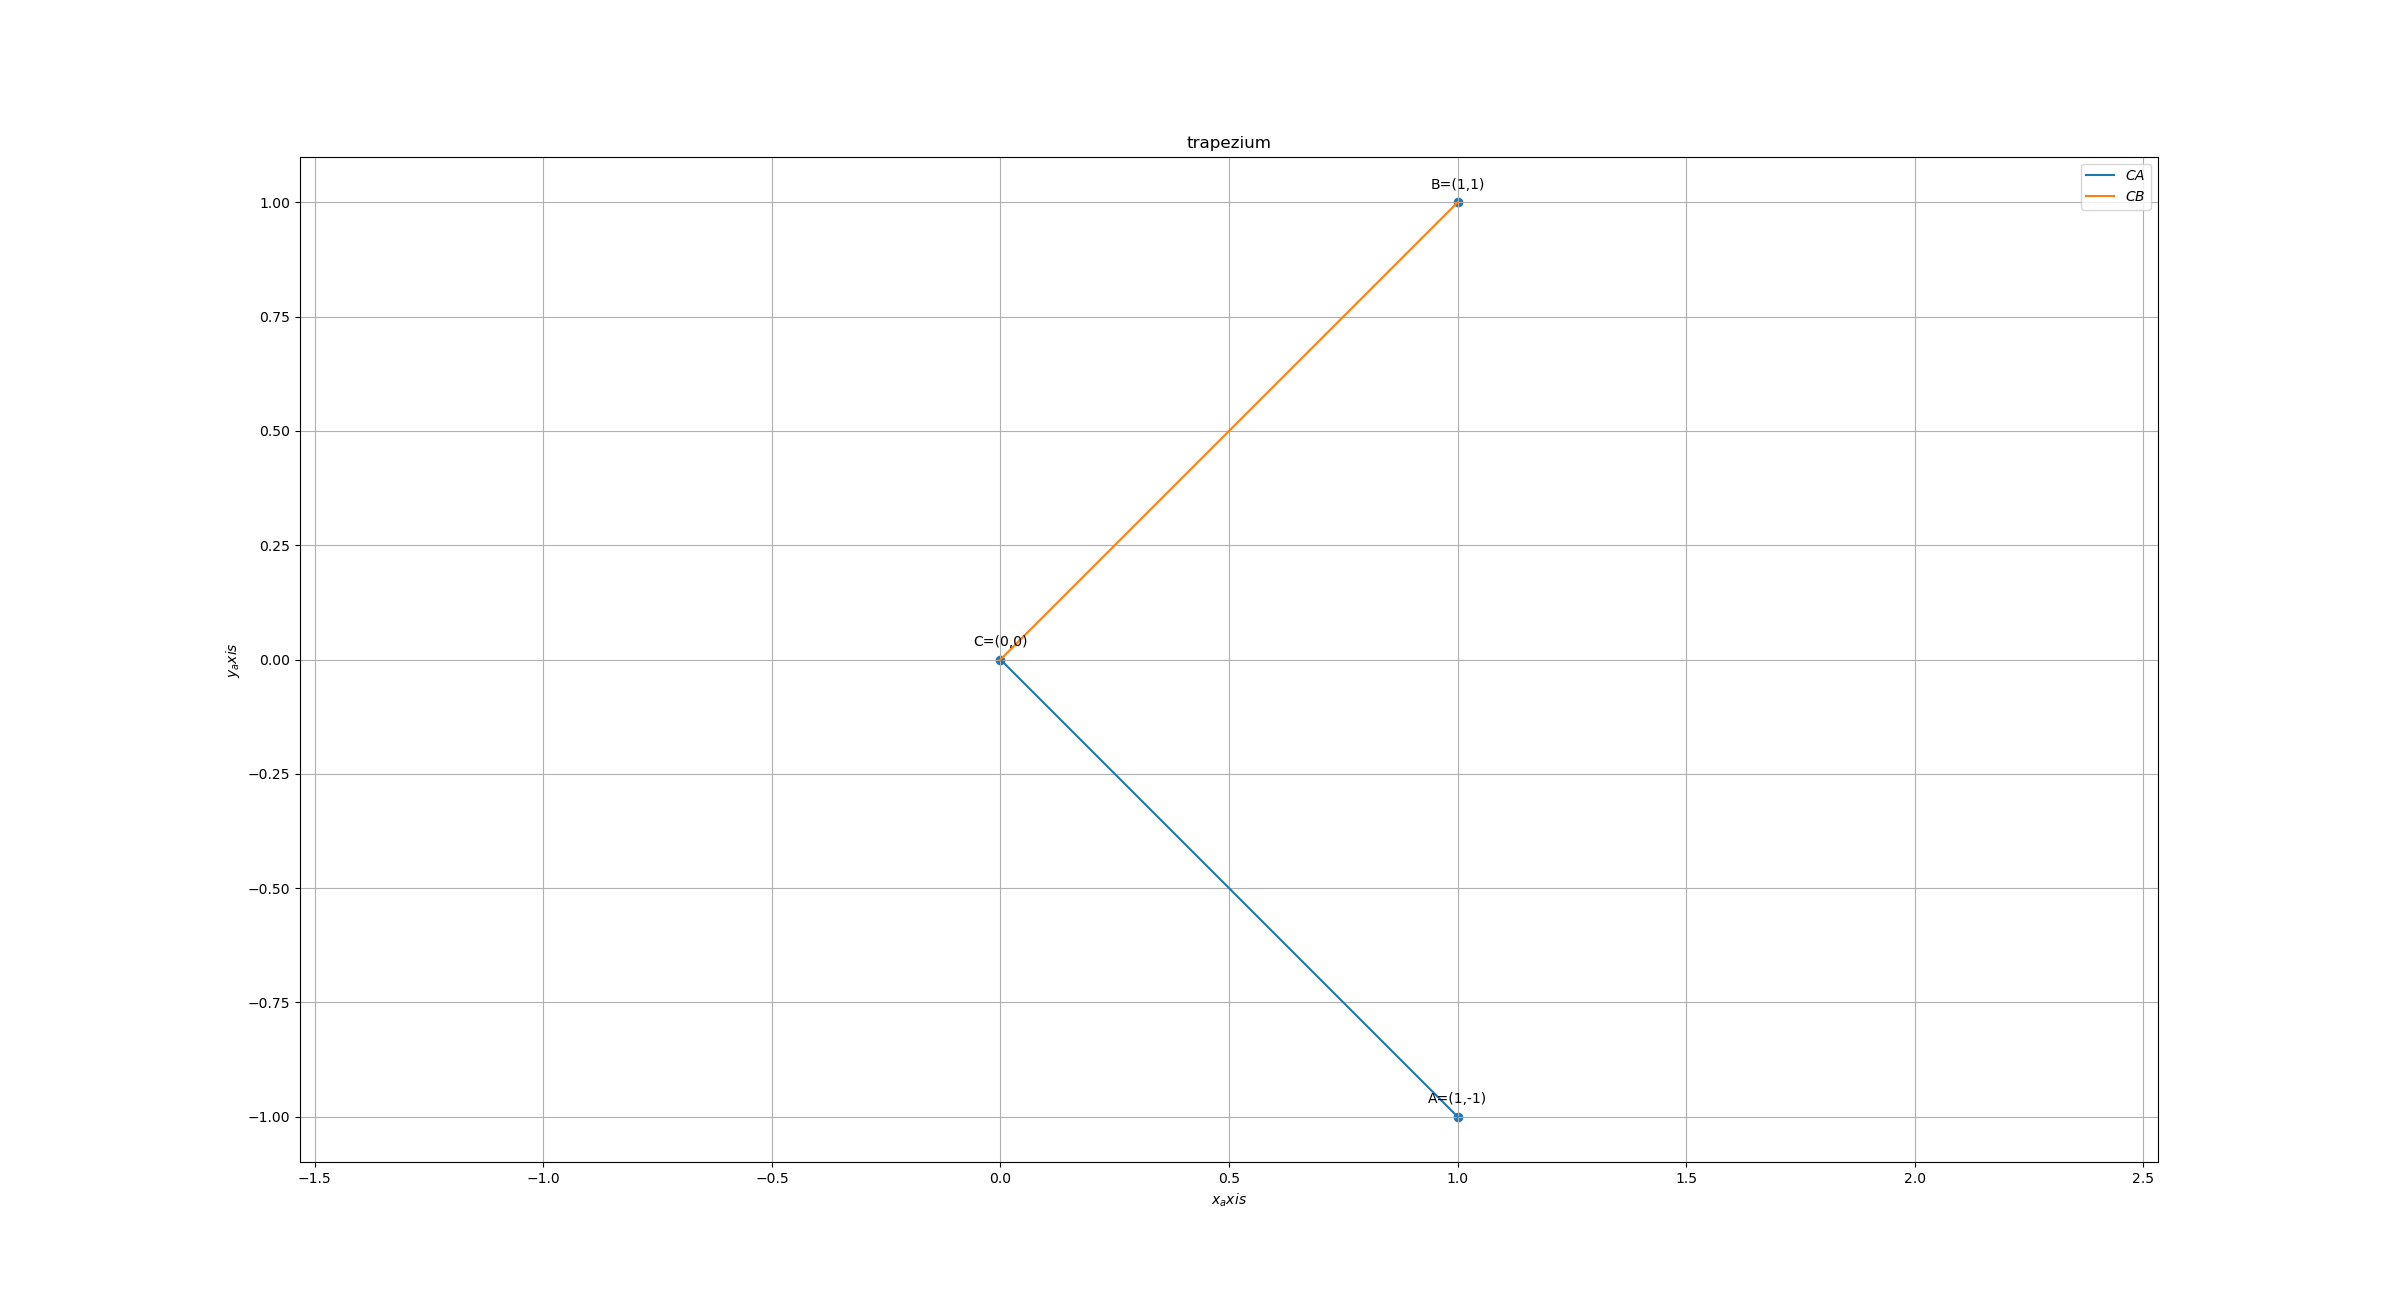
\includegraphics[width=\columnwidth]{chapters/12/10/3/3/figs/vector.png}
\caption{}
		\label{fig:12/10/3/3Figure}
\end{figure}

\item Find the projection of the vector $\hat{i}+3\hat{j}+7\hat{k}$ on the vector $7\hat{i}-\hat{j}+8\hat{k}$.
\item Show that each of the given three vectors is a unit vector: 

 $\frac{1}{7}(2\hat{i}+3\hat{j}+6\hat{k}),\frac{1}{7}(3\hat{i}-6\hat{j}+2\hat{k}),\frac{1}{7}(6\hat{i}+2\hat{j}-3\hat{k}$)
 
Also,show that they are mutually perpendicular to each other.
\item Find $\abs{\overrightarrow {a}}$ and $\abs{\overrightarrow {b}}$,if ($\overrightarrow {a}+\overrightarrow {b}).(\overrightarrow {a}-\overrightarrow {b})=8$ and $\abs{\overrightarrow {a}}=8\abs{\overrightarrow {b}}$.
\item Evaluate the product(3$\overrightarrow {a}-5\overrightarrow {b}).(2\overrightarrow {a}+7\overrightarrow {b}$).
\item Find the magnitude of two vectors $\overrightarrow {a}$ and $\overrightarrow {b}$, having the same magnitude and such that the angle between them is $60\degree$ and their scalar product is $\frac{1}{2}$
\item Find $\abs{\overrightarrow {x}}$,if for a unit vector $\overrightarrow {a},(\overrightarrow {x}-\overrightarrow {a}).(\overrightarrow {x}+\overrightarrow {a}$)=12.
	\\
		\iffalse
\documentclass[12pt]{article}
\usepackage{graphicx}
%\documentclass[journal,12pt,twocolumn]{IEEEtran}
\usepackage[none]{hyphenat}
\usepackage{graphicx}
\usepackage{listings}
\usepackage[english]{babel}
\usepackage{graphicx}
\usepackage{caption} 
\usepackage{hyperref}
\usepackage{booktabs}
\usepackage{array}
\usepackage{amsmath}   % for having text in math mode
\usepackage{listings}
\lstset{
  frame=single,
  breaklines=true
}
  
%Following 2 lines were added to remove the blank page at the beginning
\usepackage{atbegshi}% http://ctan.org/pkg/atbegshi
\AtBeginDocument{\AtBeginShipoutNext{\AtBeginShipoutDiscard}}
%


%New macro definitions
\newcommand{\mydet}[1]{\ensuremath{\begin{vmatrix}#1\end{vmatrix}}}
\providecommand{\brak}[1]{\ensuremath{\left(#1\right)}}
\providecommand{\norm}[1]{\left\lVert#1\right\rVert}
\newcommand{\solution}{\noindent \textbf{Solution: }}
\newcommand{\myvec}[1]{\ensuremath{\begin{pmatrix}#1\end{pmatrix}}}
\let\vec\mathbf

\begin{document}

\begin{center}
\title{\textbf{Vector Dot Product}}
\date{\vspace{-5ex}} %Not to print date automatically
\maketitle
\end{center}
\setcounter{page}{1}

\section{12$^{th}$ Maths - Chapter 10}
This is Problem-9 from Exercise 10.3
\begin{enumerate}
\item Find $\norm{\vec{x}}$, if for a unit vector $\vec{a}$, $\brak{\vec{x}-\vec{a}}.\brak{\vec{x}+\vec{a}} = 12$.\\
	\fi
\solution 
From the given information,
\begin{align}
  \label{eq:12/10/3/9det2f}
  \brak{\vec{x}-\vec{a}}^\top\brak{\vec{x}+\vec{a}} &= 12 \\
  \implies \vec{x}^\top\vec{x} - \vec{a}^\top\vec{x} + \vec{x}^\top\vec{a} - \vec{a}^\top\vec{a} &= 12 \\
  \implies \norm{\vec{x}}^{2} - \norm{\vec{a}}^{2} &= 12 \\
\implies   \norm{\vec{x}}^{2} - 1 &= 12  \\
	\text{or, }  
	\norm{\vec{x}} &= \sqrt{13}
\end{align}

\item If $\overrightarrow {a}=2\hat{i}+2\hat{j}3\hat{k},\overrightarrow {b}=\hat{-i}+2\hat{j}+\hat{k}$ and $\overrightarrow {c}=3\hat{i}+\hat{j}$ are such that $\overrightarrow {a}+\lambda\overrightarrow {b}$ is perpendicular to $\overrightarrow {c}$,then find the value of $\lambda$.
	\\
		\iffalse
\documentclass[12pt]{article}
\usepackage{graphicx}
\usepackage{amsmath}
\usepackage{mathtools}
\usepackage{gensymb}

\newcommand{\mydet}[1]{\ensuremath{\begin{vmatrix}#1\end{vmatrix}}}
\providecommand{\brak}[1]{\ensuremath{\left(#1\right)}}
\providecommand{\norm}[1]{\left\lVert#1\right\rVert}
\newcommand{\solution}{\noindent \textbf{Solution: }}
\newcommand{\myvec}[1]{\ensuremath{\begin{pmatrix}#1\end{pmatrix}}}
\let\vec\mathbf

\begin{document}
\begin{center}
\textbf\large{CHAPTER-10 \\ VECTOR ALGEBRA}

\end{center}
\section*{Excercise 10.3}

Q10.If $\vec{a} = 2\hat{i}+2\hat{j}+3\hat{k}, \vec{b} = -\hat{i}+2\hat{j}+\hat{k} \text{ and } \vec{c} = 3\hat{i}+\hat{j}$ are such that $\vec{a}+\lambda \vec{b}$ is perpendicular to $\vec{c}$, then find the value of $\lambda$.
\fi
\solution
Given that
\begin{align}
	(\vec{a}+\lambda \vec{b})^{\top} \vec{c} &= 0\\
\implies \vec{a}^{\top}\vec{c}+\lambda \vec{b}^{\top}\vec{c}&=0\\
\implies 	\lambda \vec{b}^{\top}\vec{c}&=-\vec{a}^{\top}\vec{c}\\
\implies 	\lambda(\vec{b}^{\top}\vec{c})(\vec{b}^{\top}\vec{c})^{-1}&=-(\vec{a}^{\top}\vec{c})(\vec{b}^{\top}\vec{c})^{-1}\\
\implies 	\lambda&=-(\vec{a}^{\top}\vec{c})(\vec{b}^{\top}\vec{c})^{-1}
\end{align}
Now substituting the values
\begin{align}
	\vec{a}^{\top}\vec{c}&=\myvec{2&2&3} \myvec{3\\1\\0} = 8\\
	\vec{b}^{\top}\vec{c}&=\myvec{-1&2&1} \myvec{3\\1\\0} = -1,
\end{align}
\begin{align}
	\lambda&=-(\vec{a}^{\top}\vec{c})(\vec{b}^{\top}\vec{c})^{-1}\\
	&=-(8)(-1)^{-1}\\
	&=8
\end{align}



\item Show that $\abs {\overrightarrow {a}}\overrightarrow {b}+\abs{\overrightarrow {b}}\overrightarrow {a}$ is perpendicular to $\abs{\overrightarrow {a}} \overrightarrow {b}-\abs{\overrightarrow {b}} \overrightarrow {a}$, for any two nonzero vectors $\overrightarrow {a}$ and $\overrightarrow {b}$.
\item If $\overrightarrow {a}.\overrightarrow {a}$=0 and $\overrightarrow {a}.\overrightarrow {b}$=0, then what can be conculded about the vector $\overrightarrow {b}$?
\item If $\overrightarrow {a},\overrightarrow {b},\overrightarrow {c}$ are unit vectors such that $\overrightarrow {a}+\overrightarrow {b}+\overrightarrow {c}=\overrightarrow {0}$, find the value of $\overrightarrow {a}.\overrightarrow {b}+\overrightarrow {b}.\overrightarrow {c}+\overrightarrow {c}.\overrightarrow {a}$.
\item If either vector $\overrightarrow {a}=0$ or $\overrightarrow {b}=0$, then $\overrightarrow {a}.\overrightarrow {b}$=0. But the converse need not be true .Justify your answer with an example.
\item If the vertices A,B,C of a triangle ABC are (1,2,3),(-1,0,0)(0,1,2), respectively , then find  $\angle{ABC}. [\angle{ABC}$ is the angle between the vectors $\overrightarrow{BA}$ and $\overrightarrow{BC}$].
\item show that the points A(1,2,7),B(2,6,3)and C(3,10,-1) are collinear.
\item show that the vectors $2\hat{i}-\hat{j}+\hat{k},\hat{i}-3\hat{j}-5\hat{k}$ and  $3\hat{i}-4\hat{j}-4\hat{k}$ from the vertices of a right angled triangle.
\item If $\overrightarrow {a}$ is a nonzero vector of magnitude 'a' and $\lambda$ a nonzero scalar , then $\lambda\overrightarrow {a}$ is unit vector if

\begin{enumerate} 
\item $\lambda=1$ 
\item $\lambda=-1$
\item $a=\abs{\lambda}$
\item $a=1/\abs{\lambda}$  
\end{enumerate}
\iffalse
\item If $\overrightarrow {a}=2\hat{i}+2\hat{j}3\hat{k},\overrightarrow {b}=\hat{-i}+2\hat{j}+\hat{k}$ and $\overrightarrow {c}=3\hat{i}+\hat{j}$ are such that $\overrightarrow {a}+\lambda\overrightarrow {b}$ is perpendicular to $\overrightarrow {c}$,then find the value of $\lambda$.
	\\
		\iffalse
\documentclass[12pt]{article}
\usepackage{graphicx}
\usepackage{amsmath}
\usepackage{mathtools}
\usepackage{gensymb}

\newcommand{\mydet}[1]{\ensuremath{\begin{vmatrix}#1\end{vmatrix}}}
\providecommand{\brak}[1]{\ensuremath{\left(#1\right)}}
\providecommand{\norm}[1]{\left\lVert#1\right\rVert}
\newcommand{\solution}{\noindent \textbf{Solution: }}
\newcommand{\myvec}[1]{\ensuremath{\begin{pmatrix}#1\end{pmatrix}}}
\let\vec\mathbf

\begin{document}
\begin{center}
\textbf\large{CHAPTER-10 \\ VECTOR ALGEBRA}

\end{center}
\section*{Excercise 10.3}

Q10.If $\vec{a} = 2\hat{i}+2\hat{j}+3\hat{k}, \vec{b} = -\hat{i}+2\hat{j}+\hat{k} \text{ and } \vec{c} = 3\hat{i}+\hat{j}$ are such that $\vec{a}+\lambda \vec{b}$ is perpendicular to $\vec{c}$, then find the value of $\lambda$.
\fi
\solution
Given that
\begin{align}
	(\vec{a}+\lambda \vec{b})^{\top} \vec{c} &= 0\\
\implies \vec{a}^{\top}\vec{c}+\lambda \vec{b}^{\top}\vec{c}&=0\\
\implies 	\lambda \vec{b}^{\top}\vec{c}&=-\vec{a}^{\top}\vec{c}\\
\implies 	\lambda(\vec{b}^{\top}\vec{c})(\vec{b}^{\top}\vec{c})^{-1}&=-(\vec{a}^{\top}\vec{c})(\vec{b}^{\top}\vec{c})^{-1}\\
\implies 	\lambda&=-(\vec{a}^{\top}\vec{c})(\vec{b}^{\top}\vec{c})^{-1}
\end{align}
Now substituting the values
\begin{align}
	\vec{a}^{\top}\vec{c}&=\myvec{2&2&3} \myvec{3\\1\\0} = 8\\
	\vec{b}^{\top}\vec{c}&=\myvec{-1&2&1} \myvec{3\\1\\0} = -1,
\end{align}
\begin{align}
	\lambda&=-(\vec{a}^{\top}\vec{c})(\vec{b}^{\top}\vec{c})^{-1}\\
	&=-(8)(-1)^{-1}\\
	&=8
\end{align}



\item Show that $\abs {\overrightarrow {a}}\overrightarrow {b}+\abs{\overrightarrow {b}}\overrightarrow {a}$ is perpendicular to $\abs{\overrightarrow {a}} \overrightarrow {b}-\abs{\overrightarrow {b}} \overrightarrow {a}$, for any two nonzero vectors $\overrightarrow {a}$ and $\overrightarrow {b}$.
\item If $\overrightarrow {a}.\overrightarrow {a}$=0 and $\overrightarrow {a}.\overrightarrow {b}$=0, then what can be conculded about the vector $\overrightarrow {b}$?
\item If $\overrightarrow {a},\overrightarrow {b},\overrightarrow {c}$ are unit vectors such that $\overrightarrow {a}+\overrightarrow {b}+\overrightarrow {c}=\overrightarrow {0}$, find the value of $\overrightarrow {a}.\overrightarrow {b}+\overrightarrow {b}.\overrightarrow {c}+\overrightarrow {c}.\overrightarrow {a}$.
\item If either vector $\overrightarrow {a}=0$ or $\overrightarrow {b}=0$, then $\overrightarrow {a}.\overrightarrow {b}$=0. But the converse need not be true .Justify your answer with an example.
\item If the vertices A,B,C of a triangle ABC are (1,2,3),(-1,0,0)(0,1,2), respectively , then find  $\angle{ABC}. [\angle{ABC}$ is the angle between the vectors $\overrightarrow{BA}$ and $\overrightarrow{BC}$].
\item show that the points A(1,2,7),B(2,6,3)and C(3,10,-1) are collinear.
\item show that the vectors $2\hat{i}-\hat{j}+\hat{k},\hat{i}-3\hat{j}-5\hat{k}$ and  $3\hat{i}-4\hat{j}-4\hat{k}$ from the vertices of a right angled triangle.
\item If $\overrightarrow {a}$ is a nonzero vector of magnitude 'a' and $\lambda$ a nonzero scalar , then $\lambda\overrightarrow {a}$ is unit vector if

\begin{enumerate} 
\item $\lambda=1$ 
\item $\lambda=-1$
\item $a=\abs{\lambda}$
\item $a=1/\abs{\lambda}$  
\end{enumerate}
\fi

\end{enumerate}

